%\documentclass[]{acmtrans2m}
%\documentclass[acmtoms,acmnow]{acmtrans2m}
\documentclass[12pt]{article}
%\usepackage{utopia}     % Use Utopia font
\usepackage{txfonts}     % Use Utopia font
\usepackage{html}
\usepackage{url}
\usepackage{natbib}
\usepackage[dvips]{graphicx, color}  % The figure package

%\acmYear{03}
%\acmMonth{11}

%\newtheorem{theorem}{Theorem}[section]
%\newtheorem{conjecture}[theorem]{Conjecture}
%\newtheorem{corollary}[theorem]{Corollary}
%\newtheorem{proposition}[theorem]{Proposition}
%\newtheorem{lemma}[theorem]{Lemma}
%\newdef{definition}[theorem]{Definition}
%\newdef{remark}[theorem]{Remark}

\setlength{\textheight}{22.0cm}
\setlength{\textwidth}{16.00cm}
\setlength{\topmargin}{-0.5cm}
\setlength{\oddsidemargin}{0.0cm}
\setlength{\evensidemargin}{0.5cm}
\setlength{\parskip}{5pt}
\setlength{\parindent}{20pt}

\newcommand{\Fussy}{{\tt fussy}}
\newcommand{\DS}{{\tt DS}}
\newcommand{\VMS}{{\tt VMS}}
\def\runningfoot{\def\@runningfoot{}}
\def\firstfoot{\def\@firstfoot{}}
           
\markboth{S. Bhatnagar}{Automatic random error propagation}


\begin{document}
\title{The {\tt fussy} language: Implementation of an automatic
error propagation algorithm}
\author{S. Bhatnagar \\National Radio Astronomy Observatory}
\date{Nov. 2003}
\maketitle
\begin{center}
\htmladdnormallinkfoot{[PDF version]}{http://www.aoc.nrao.edu/~sbhatnag/Softwares/fussy/fussy.pdf}
\end{center}

\begin{abstract} 
Formal propagation of random errors in a mathematical expression
follow a precise prescription based on calculus.  This requires the
computation of the variation of the function with respect to each of
the independent variables used to construct the function.  These
variations are added in quadrature to compute the final numerical
error.  For complicated expressions, computation of all the partial
derivatives is often cumbersome and hence error prone.

The \Fussy\footnote{The name reflects the original intention of
  designing a language for fuzzy arithemetic.  It is also a pun on
  those who (wrongly) consider error propagation as too much fuss!}
scripting language, described here, implements an algorithm for
automatic propagation of random measurement errors in an arbitrary
mathematical expression.  It is internally implemented as a virtual
machine for efficient runtime performance and can be used as an
interpreter by the user.  A simple {\tt C} binding to the interpreter
is also provided.  Mathematical expressions can be implemented as a
collection of sub-expressions, as sub-program units (functions or
procedures) or as single atomic expressions.  Errors are correctly
propagated when a complex expression is broken up into smaller
sub-expressions.  Sub-expressions are assigned to temporary variables
which can then be used to write the final expression.  These temporary
variables are not independent variables and the information about
their dependence on other constituent independent variables is
preserved and used on-the-fly in error propagation.

The scripting syntax of \Fussy\ is similar to that of {\tt C}.  It is
therefore easy to use with minimal learning and can be used in every
day scientific work.  Most other related work found in the literature
is in the form of libraries for automatic differentiation.  Only two
tools appear to have used it for automatic error propagation.  Use of
these libraries and tools require sophisticated programing and are
targeted more for programmers than for regular every day scientific
use.  Also, such libraries and tools are difficult to use for correct
error propagation in expressions composed of sub-expressions.
\end{abstract}
            
%\category{D.0}{Software}{General}[Automatic error propagation]
            
%\terms{Algorithms}
            
%\keywords{Automatic random error propagation, random variables}
            
%\begin{bottomstuff} 
%Author's address: P.O. Box 'O', Socorro, New Mexico-87801, USA.\\
%E-mail address: {\tt sbhatnag@aoc.nrao.edu} \\ Associated Universities
%Inc. operates the National Radio Astronomy Observatory under
%cooperative agreement with the National Science Foundation.
%\end{bottomstuff}
            

\section{Introduction}

If $\vec x$ is a vector of independent experimentally measured
quantities with associated random measurement error $\delta \vec
x$, the formal error on a function $f(\vec x)$ is given by
\begin{equation}
  \delta f = \sqrt{\sum_i {\left( {\partial f \over {\partial x_i}} 
        \delta x_i \right)}^2}
\label{FERR}
\end{equation}
Further, if $f(\vec x)$ is a functional, e.g. $f(\vec x)=g(h(k(\vec
x)))$, then the partial derivative of $f$ is given by the derivative
chain rule:
\begin{equation}
{\partial f \over \partial x_i} = {\partial f \over \partial h} 
{\partial h \over \partial k} {\partial k \over \partial x_i}
\label{DFUNCTIONAL}
\end{equation}
Therefore, for the computation of $\delta f$, one requires:
\begin{enumerate}
\item the partial derivative of the function with respect to each
independent variable ($\partial f / \partial x_i$)
\item $\delta x_i$ - the measurement error
\item chain rules of differential calculus for the
mathematical operators (which will use the $x_i$'s and $\partial f /
\partial x_i$'s).  
\end{enumerate}

In the following sections, the implementation of an algorithm for
automatic computation of partial derivatives and propagation of random
errors in an arbitrary mathematical expression is described.  The
algorithm is implemented as a scripting language called \Fussy\ and
can be used as an interpreter by the user.  The syntax is similar to
that of the {\tt C} language making it easy to use in an interactive
session or as a scripting environment.  Each user defined variable in
\Fussy\ is treated as an independent variable and expressions can be
constructed using an arbitrary number of variables.  It is error prone
to express complicated expressions as single atomic statements and
usually the final expression is built out of sub-expressions and
temporary variables.  For the purpose of random error propagation
however, temporary variables are dependent on the independent
variables (normal user defined variables) on the right hand side of an
assignment operator.  The algorithm described below does correct error
propagation in the final expression composed of such temporary
variables.  A special language feature is used to distinguish between
such temporary and normal variables as well as to associate
measurement errors with numbers (see
Appendix~\ref{APPEN:SYNTAX_EXPR}).

Although it is possible to code Eq.~\ref{FERR} in other tools
\citep{Calc,EDA,Bischof1997A-A}, it requires sophisticated programing
and learning often arcane, new programing tools.  This is usually time
consuming and enough of a bother to discourage its use for the purpose
of error propagation in every-day scientific use.  The work of
\citet{Stoutemyer:1977} using the {\tt REDUCE} algebraic manipulation
language \citep{REDUCE2,REDUCE} was one of the first which used
automatic symbolic differentiation for error analysis in {\it single
  atomic mathematical expressions}.  \citet{EDA} has used a similar
approach and developed a tool for {\tt
  Mathematica}\footnote{\copyright 2003 Wolfram Research, Inc.}.
There are program development libraries
\citep{ScComp,Griewank:1996:AAP,Tsukanov2003Dsa} for automatic
differentiation which could be used for similar purpose.  However they
too suffer from the same problem of requiring more effort from the
user than is possible in everyday work.  Besides, most of these
existing tools will be hard to use for multi-variate expressions and
functionals.  They are even harder (if not impossible) to use directly
for complicated expressions expressed as a combination of
sub-expressions.  Apart from the difficulty of use, the two tools
which do use automatic differentiation for error propagation require
access and familiarity with other packages (the {\tt REDUCE} package
or the commercially sold package {\tt Mathematica}).

The \Fussy\ interpreter is implemented internally as a virtual machine
(VM) with a stack of its own.  The derivative chain rule
(Eq.~\ref{DFUNCTIONAL}) is implemented using a separate VM which has a
separate stack {\it per independent variable} to hold the intermediate
partial derivatives.  At the terminal nodes of a parsing tree (e.g.
the '{\tt =}' operator) the values from these stacks are used to
evaluate Eq.~\ref{FERR}.  A user program written in \Fussy\ is
compiled into the VM instruction-set, referred to as the op-codes, to
manipulate the VM stack (\VMS), call built-in functions, perform basic
mathematical operations or call user defined sub-program (functions or
procedures).  These op-codes are function calls which perform the
operation they represent (mathematical operators, built-in function
call or branching to a sub-program unit) as well as the steps required
for automatic error propagation.  Since user defined
programs/expressions are translated into these op-codes, errors are
correctly propagated in the mathematical expression in any arbitrary
user program.

A simple {\tt C} binding to the interpreter is also provided.  The
user program can be supplied to the interpreter via an in-memory
string using the function {\tt calc(char} {\tt *InString,} {\tt
edouble} {\tt \&ans,} {\tt FILE} {\tt *InStream,} {\tt FILE} {\tt
*OutStream)}.  The contents of the {\tt InString} are parsed and
converted to a VM instruction set.  The result of the execution of
this program is returned in {\tt ans}.  The last two arguments are not
used in this case.  Alternatively, if {\tt InString} is set to {\tt
NULL} and the last two arguments set to valid file pointers, the
interpreter will take the input from {\tt InFile} and use {\tt
OutFile} as the output stream.  A similar {\tt C++} interface of type
{\tt calc(}{\tt char *InString,} {\tt ostream \&ResultStream,} {\tt
FILE *InStream,} {\tt FILE *OutStream)} writes the result of the
program supplied in {\tt InString} or via the file pointer {\tt
InStream} to the output stream {\tt ResultStream}.  {\tt OutStream} in
both interfaces is used as the output file for the error messages.

For a better understanding, in Section~\ref{SEC:SINGLE_VAR} I describe
the algorithm for automatic random error propagation for the simpler
case of a single variate expression.  Section~\ref{SEC:MULTI_VAR}
describes the complete algorithm, along with the logic for the various
operators in the form of pseudo code.  The correctness of the
algorithm is demonstrated in Section~\ref{SEC:EXAMPLES} using
numerical examples.  On the lines of proof of correctness of the
algorithm, it is also argued that the algorithm is general and will
work for any arbitrary expression.  In Appendix~\ref{APPEN:EX}, a
step-wise description of the algorithm for a general mathematical
expression is given.  Appendix~\ref{APPEN:SYNTAX} describes the syntax
of the \Fussy\ language.

\section{Error propagation: Single variable case}
\label{SEC:SINGLE_VAR}

For the case where $f$ is a function of a single measurable $x$, the
right hand side of Eq.~\ref{FERR} can be evaluated as follows.  Each
leaf of the parsing tree will either be (1) a constant, (2) a
variable, or (3) another sub-tree representing a sub-expression.  The
derivatives can be computed by the repeated application of the
derivative chain rule.  Starting from the bottom of the tree, a value
of $1$ is pushed on the Derivative Stack (\DS) (equivalent of putting
$\partial x / \partial x$ on the stack) for every leaf of the tree
(which, at the bottom, correspond to the symbols from the symbol
table or constants).  The nodes of a tree corresponds to one of the
arithmetic operators ('{\tt +}', '{\tt -}', '{\tt /}', '{\tt *}',
'{\texttt {\^}}', and '{\tt **}') or built-in functions, which are
implemented as function calls.  These functions push the result of the
operations on the \VMS\ while the corresponding partial derivatives
are pushed on the \DS.

The final result and the error propagation will in general use the
values from both the stacks (the \VMS\ and the \DS).  E.g. for
$f(x)=\sin(x)*\cos(x)$, when the execution reaches the node for the
'$*$' operator, the \VMS\ will have two values, namely $\sin(x)$ and
$\cos(x)$.  The \DS\ also has two values, namely the two derivatives
$\partial \sin(x) / \partial x = \cos(x)$ and $\partial \cos(x) /
\partial x = -\sin(x)$.  The value of $f$ is pushed on the \VMS,
and its derivate ($\partial \sin(x) / \partial x * \cos(x) + \sin(x) *
\partial \cos(x) / \partial x$), computed using both the stacks, pushed
on the \DS.  The '{\tt =}' operator rule finally takes the value from
the \DS, and compute the right hand side of Eq.~\ref{FERR}.

An arbitrary expression composed of user defined variables or built-in
functions, will itself be represented as a sub-tree.  Hence, applying
the above algorithm recursively, case (3) above (a sub-expression)
will also be correctly handled.

\subsection{Example}
\begin{figure}[t]
\begin{center}
  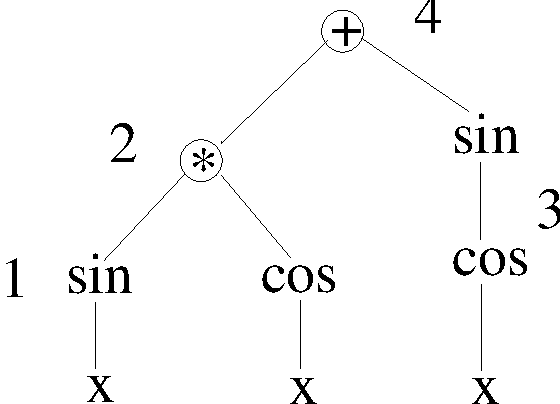
\includegraphics[scale=0.45]{Figs/fig1}
\caption[]{The parsing tree for the expression $f(x)=\sin(x)*\cos(x) + \sin(\cos(x))$}
\label{EX1}
\end{center}
\end{figure}
Let $f(x)=\sin(x)*\cos(x) + \sin(\cos(x))$ (this includes three
sub-expressions one of which is a functional), represented as a tree
in Fig.~\ref{EX1}.  A value of $1$ is pushed on the \DS\ whenever a
symbol from the symbol-table is pushed on the \VMS.  When branch {\bf
1} in the above tree is reduced, a call to the built-in function
$\sin$ pops a value from the \VMS\ (which is $x$) and a value from the
\DS\ (say $dx$, which is $1$).  It then pushes the value of $\sin(x)$
on the \VMS\ and a value of $dx*\partial \sin(x) / \partial x =
1*\cos(x)$ on the \DS.  Similar operations are done for evaluating
$\cos(x)$.  When the execution reaches node {\bf 2}, the \VMS\ has the
values $\sin(x)$ ({\tt L}) and $\cos(x)$ ({\tt R}) and the \DS\ has
$\cos(x)$ ({\tt dL}) and $-\sin(x)$ ({\tt dR}).  Since '$*$' is a
binary operator, when node {\bf 2} is reduced, two values each from
the \VMS\ and the \DS\ are poped.  The multiplication operator then
pushes {\tt L*R}=$\sin(x)*\cos(x)$ on the \VMS\ while {\tt L*dR +
R*dL}=$\cos^2(x)-\sin^2(x)$ is pushed on the \DS\ (note that this uses
values from the \DS\ as well as from the VMS).  Both the stacks now
have one value each - \VMS\ the value of the sub-expression
$\sin(x)*\cos(x)$ and the \DS\ the value of the derivative of this
sub-expression.

Next, branch {\bf 3} is evaluated.  Again, $1$ and $x$ are pushed on
the \DS\ and the \VMS\ respectively.  A call to $\cos$ compute the
derivative of $\cos(x)$ (namely, $-\sin(x)$) and multiplies it by the
top of the \DS\ (which is $1$).  When call for $\sin$ is made, its
argument ($\cos(x)$) and the derivative of the argument are on the
\DS\ and \VMS\ respectively. A value from the \VMS\ and \DS\ each (say
{\tt L}=$\cos(x)$ and {\tt dL} =$-\sin(x)$) respectively) are poped.
$\sin(L)=\sin(\cos(x))$ and {\tt dL}$*\sin(L)=-\sin(x)*\sin(\cos(x))$
are pushed on the \VMS\ and \DS\ respectively.  This is the equivalent
of Eq.~\ref{DFUNCTIONAL} for branch {\bf 3}.  At this stage, the two
values on the \VMS\ are the values of the two sub-expression and \DS\
has the values of the partial derivatives of the two sub-expressions.

Reduction of the node {\bf 4} will then again invoke the rule for the
derivative and the binary operator for addition: pop two values each
from the \VMS\ and \DS, push the result of the operator on the \VMS,
and the derivative ({\tt dL+dR} in this case) on the \DS.  Top of the
\DS\ now has $\partial f / \partial x$ and the '{\tt=}' operator
computes Eq. \ref{FERR}.

\section{Error propagation: Algorithm for the multi-variate case}
\label{SEC:MULTI_VAR}

The algorithm for the multi-variate case is similar to the
single-variate case described above, but slightly more complicated.
Multi-variate expressions have the added complication that the terms
in the summation of Eq.~\ref{FERR} have to be evaluated separately for
{\it each independent} variable.  This means that a \DS\ and a table
of measurement errors ({\tt ME}) {\it per independent} variable have
to be maintained.

Symbols (variables and constants) in \Fussy\ are tagged with a number
or a list of numbers (the IDs) and a type.  Symbols representing
normal variables are of the type {\tt VAR} and have a single unique
ID, a random error and a partial derivative (of value 1) associated
with them.  Symbols representing sub-expressions are of the type {\tt
PARTIAL\_VAR} and have a list of IDs and a corresponding list of
random errors and partial derivatives associated with them.  List of
unique IDs and the random errors of the independent variables in the
expression on the right-hand side (RHS) of the assignment operator
constitute the list of IDs and random errors for the {\tt
PARTIAL\_VAR} type symbols.  When a symbol (of either type) is pushed
on the \VMS, the entire list of associated IDs is copied to the ID
list of the object on the stack.  The corresponding random errors and
partial derivatives are also copied in the appropriate locations in
the {\tt ME} table and pushed on the appropriate \DS\ respectively.
For example, let the IDs of $x_1$ and $x_2$ be $1$ and $2$
respectively.  The result of $x_1 * x_2$ on the top of the \VMS\ will
have an ID list of {\tt \{1,2\}} retaining the information that the
result is statistically dependent on the independent variates $x_1$
and $x_2$.  If this result is further used as part of another
expression, this information will be used to propagate the chain rule
for these variables correctly.

Since any expression is built using basic mathematical operators or
built-in functions, for the purpose of proving the correctness of the
error propagation algorithm for any arbitrary expression, it is
sufficient to prove that the algorithm works for the fundamental
mathematical operators and built-in functions.  The algorithms for
evaluating the partial derivatives involving mathematical operators
and the final evaluation of the resulting error is described below as
pseudo code (see Appendix~\ref{APPEN:EX} for an example).  The
algorithms are described using the following pseudo functions:
\begin{itemize}
\item {\tt push(S)}: to push the symbol or value {\tt S} on the \VMS. 
\item {\tt push(S,DS[i])}: to push the symbol or value {\tt S} on the
$i^{th}$ \DS.  
\item {\tt pop()}: to pop a symbol from the \VMS.
\item {\tt Top(DS[i])}:  represents the value on the top of the
$i^{th}$ \DS. 
\end{itemize}
The \DS\ is indexed by the symbol ID(s) (say, {\tt N}).  When a symbol
from one of the symbol tables is pushed on the \VMS, a value of $1$ is
pushed on {\tt DS[N]} and the associated measurement error is copied
into {\tt ME[N]}.  {\tt L} and {\tt R} in the pseudo code represents
the symbols on the left-hand-side (LHS) and right-hand side (RHS) of
the operator respectively.  Two functions $f(x,a)$ and $g(x,b)$ with
one common variable ($x$) and one non-common variable each ($a$ and
$b$) are used as the LHS and RHS operands in the explanation below.

All the operators described below are binary operators.  They all pop
two values from the top of the \VMS, compute the result by applying
the corresponding operator, store the value in a temporary stack
object, set its ID to the union of the IDs of the operands and push it
on the \VMS.  These operations are performed by the following pseudo
function:
\begin{verbatim}
   ComputeResult(L,R,Expr)
     {
         L = pop();     R = pop();
         S = Expr(L,R);
         S.IDList = union(L.IDList,R.IDList);
         push(S);
     }
\end{verbatim}
{\tt Expr} implements the arithmetic of the mathematical operation on
{\tt L} and {\tt R}. 

%{\tt dCommonExpr} below represents the operations required for
%computing the derivative with respect to the common IDs between the
%operands and {\tt CommonExpr} returns the actual value of the partial
%derivative (${f(x,a)} {\partial g(x,b) \over
%\partial x} + {g(x,b)}{\partial f(x,a) \over \partial x}$).  {\tt
%dNoncommonVar} represents the operations for the derivative with
%respect to the non-common IDs and {\tt LExpr} and {\tt RExpr} returns
%the values of these derivatives for the left- and right-hand side
%operands respectively (${g(x,b)}{\partial f(x,a) \over \partial a}$
%and ${f(x,a)} {\partial g(x,b) \over \partial b}$).

Partial derivatives with respect to all the IDs in the ID lists of the
operands are at the top of the corresponding \DS s.  For all the IDs
common between the two operands, two values are poped from the
corresponding \DS, say {\tt dxR} and {\tt dxL}.  The common IDs
represent the variables which are part of both the operands (here
$x$).  Operations to compute the partial derivatives with respect to
these common variables (equivalent of the ${\partial \over \partial
x}$ operator) are represented by the pseudo function {\tt dCommonVar}
below.  The function {\tt CommonExpr} implements the arithmetic for
the derivative computation and is set to the appropriate function for
the various operators.  These values are computed for each ID in the
set composed of the intersection of the ID lists of the two operands,
and pushed on the corresponding \DS\ (here, the ID of $x$).  Finally,
all IDs common between the two operands are removed from the ID lists
of each operand.
\begin{verbatim}
   dCommonVar(L,R,CommonExpr) 
     { 
         IDList = intersection(L.ID,R.ID); 
         for ID in IDList 
           { 
              dxR = pop(DS[ID]); 
              dxL = pop(DS[ID]); 
              push(CommonExpr(L,R,dxL,dxR),DS[ID]);
              L.Remove(ID);  R.Remove(ID); 
           } 
     }
\end{verbatim}
The list of IDs of the two operands now has IDs corresponding to the
non-common variables only ($a$ and $b$ here).  Operations for the
partial derivatives of the operands with respect to these variables is
represented by the pseudo function {\tt dNonCommonVar} below.  {\tt
LExpr} and {\tt RExpr} computes the value of these derivatives for the
LHS and RHS of the operator (equivalent of computing $\frac{\partial
f(x,a)}{\partial a}$ and $\frac{\partial g(x,b)}{\partial b}$) using
the values from the top of the appropriate
\DS.
\begin{verbatim}
   dNonCommonVar(L,R,LExpr, RExpr)
     {
         for ID in L.IDList
            Top(DS[ID]) = LExpr(L,R,Top(DS[ID]));

         for ID in R.IDList
            Top(DS[ID]) = RExpr(L,R,Top(DS[ID]));
     }
\end{verbatim}
%\newpage
%
%--------------------------------------------------------------------  
%
\subsection{The multiplication operator}

The following code returns the result of the operator ({\tt L*R}) on
the top of the \VMS\ with an ID equal to {\tt L.ID $\cup$ R.ID}.
\begin{verbatim}
   Expr(L,R) {return L*R};  /* Compute the value for 
   ComputeResult(L,R,Expr);    the multipication operator */
\end{verbatim}
Following code returns the value(s) of the partial derivative(s) (here
{\tt dxR*L + dxL*R}) with respect to {\it all} the common variables in
the two operands, on the top of the appropriate \DS s.  
\begin{verbatim}
   Expr(L,R,dxL,dxR) {return dxR*L + dxL*R;}
   dCommonVar(L,R,Expr);
\end{verbatim}
The following code returns the value of the partial derivatives with
respect to the variables not common between the operands.  These
values are returned on the top of the \DS\ corresponding to the remaining
IDs of the two operands.
\begin{verbatim}
   LExpr(L,R,dx) {return dx*L};
   RExpr(L,R,dx) {return dx*R};
   dNoncommonVar(L,R,LExpr,RExpr)
\end{verbatim}
%
%-------------------------------------------------------------------------
%
\subsection{The division operator}

As before, the result of the division operator is computed as {\tt
L/R} and returned on the \VMS\ using the following code.
\begin{verbatim}
   Expr(L,R) {return L/R};  /* Compute the value for 
   ComputeResult(L,R,Expr);    the division operator */
\end{verbatim}
For all IDs common between {\tt L} and {\tt R}, the partial derivative
is computes as {\tt (R*dxL - L*dxR)/(R*R)} and returned on the
appropriate \DS s using the following code.  
\begin{verbatim}
   Expr(L,R,dxL,dxR) {return (R*dxL - L*dxR)/(R*R)};
   dCommonVar(L,R,Expr);
\end{verbatim}
This is equivalent to computing
\begin{equation}
{\partial \over {\partial x}}\left[{f(x,a) \over g(x,b)}\right] =
{1 \over g(x,a)^2}\left[{g(x,a) {{\partial f(x,a)} \over  {\partial
x}}} - f(x,a) {{\partial g(x,b)} \over {\partial x}}\right] 
\end{equation}
Next, partial derivatives with respect to each of the non-common
variables are computed (here with respect to $a$ as ${1 \over g(x,b)}
{\partial f(x,a) \over \partial a}$ and with respect to $b$ as
$-{f(x,a) \over {g(x,b)^2}}{\partial g(x,b) \over \partial b}$) and
returned on the appropriate \DS s by the following code.
\begin{verbatim}
   LExpr(L,R,dx) {return dx/R};
   RExpr(L,R,dx) {return -L*dx/(R*R)};
   dNoncommonVar(L,R,LExpr,RExpr);
\end{verbatim}
%
%-------------------------------------------------------------------------
%
\subsection{The addition operator}

The first set of operations is same as that for other operators except
that the value pushed on the \VMS\ is {\tt L+R}.
\begin{verbatim}
   Expr(L,R) {return L+R};  /* Compute the value for 
   ComputeResult(L,R,Expr);    the addition operator */
\end{verbatim}
Since the partial derivatives of the expression with respect to the
non-common variables is already on the appropriate \DS, no separate
operation is required for these variables.  The partial derivatives
with respect to the common set of variables is computed as ${\partial
f(x,a) \over {\partial x}}$ and ${\partial g(x,b) \over {\partial
x}}$.  The pseudo code for these operations is:
\begin{verbatim}
   Expr(L,R,dxL,dxR) {return (dxL + dxR)};
   dCommonVar(L,R,Expr);
\end{verbatim}
%
%-------------------------------------------------------------------------
%
\subsection{The subtraction operator}

The pseudo code for the subtraction operation is functionally same as
that for the addition operator.
\begin{verbatim}
   Expr(L,R) {return L-R};  /* Compute the value for the 
   ComputeResult(L,R,Expr);    subtraction operator     */

   /* Compute the derivative w.r.t. common variables */
   Expr(L,R,dxL,dxR) {return (dxL - dxR)};
   dCommonVar(Expr,L,R);
\end{verbatim}
This is equivalent of computing ${\partial f(x,a) \over {\partial
    x}}-{\partial g(x,b) \over {\partial x}}$.  In addition to the
above operations, the partial derivatives of the RHS operand with
respect to all the non-common variables needs to be negated (here
$\partial g(x,b) / \partial b$).
\begin{verbatim}
   IDList = union(L.IDList, R.IDList);
   for ID in IDList /* unique IDs in L and R */
     if (ID in R.IDList)
       {
         dxR = pop(DS[ID]);
         push(-dxR, DS[ID]);
       }
\end{verbatim}
  
%
%-------------------------------------------------------------------------
%
\subsection{The power operator}

Again, the result of the to-the-power operator ($L^R$), with an ID
equal to {\tt L.ID $\cup$ R.ID} is pushed on the \VMS\ using the code:
\begin{verbatim}
   Expr(L,R) {return L^R};  /* Compute the value for 
   ComputeResult(L,R,Expr);    the power operator */
\end{verbatim}
The partial derivative of the expression with respect to the common
variable (here $x$) is computed as:
\begin{equation}
{\partial \over {\partial
x}}\left(f(x,a)^{g(x,b)}\right)=f(x,a)^{g(x,b)} \left[{g(x,b) \over
f(x,a)} {\partial f(x,a)  \over \partial x} + \log(f(x,b)) 
{\partial g(x,b) \over \partial x} \right] 
\end{equation}
The pseudo code for this operation is:
\begin{verbatim}
   Expr(L,R,dxL,dxR) {return (L^R)*((R/L)*dxL + log(L)*dxR)};
   dCommonVar(L,R,Expr);
\end{verbatim}
The partial derivatives with respect to the non-common set of IDs
correspond to $g(x,b)f(x,a)^{[g(x,b)-1]} {\partial f(x,a) \over
{\partial a}}$ and $f(x,a)^{g(x,b)} \log(f(x,b)) {\partial g(x,b)
\over \partial b}$.  Partial derivatives of $f$ and $g$ with respect
to $a$ and $b$ are computed using the functions {\tt LExpr} and {\tt
RExpr}.  The computed partial derivatives are pushed back on the
appropriate \DS s.  The pseudo code for this operation is:
\begin{verbatim}
   LExpr(L,R,dx) {return R*(L^(R-1))*dx};
   RExpr(L,R,dx) {return (L^R)*log(L)*dx};
   dNoncommonVar(L,R,LExpr,RExpr);
\end{verbatim}
At the terminal operators (e.g. the assignment operator '{\tt =}'), a
single value (the result of the right hand side of the terminal
operator) is poped from the \VMS.  The propagated error is then
computed using the values from the top of all {\tt DS}s corresponding
to the IDs in the ID list of the poped value.  The values from these
\DS s are the partial derivatives of the expression with respect
to the various independent variables used in the expression on the
right hand side ($\partial f / \partial x_i$ in Eq.~\ref{FERR}).  The
corresponding measurement errors ($\delta x_i$ in Eq.~\ref{FERR}) are
in the appropriated locations in the {\tt ME} table.  Using these
values, Eq.~\ref{FERR} is evaluated.  This is the final propagated
error in the expression.

\section{Examples}
\label{SEC:EXAMPLES}
Following are some examples to demonstrate as well as test the
correctness of the error propagation algorithm of
Section~\ref{SEC:MULTI_VAR}.  In the following examples, various
functions are written in different algebraic forms and the results for
the different forms is shown to be exactly same (e.g. $\cos(x)$ vs.
$\sqrt{1-\sin^2(x)}$, $\tan(x)$ vs. $\sin(x)/\cos(x)$).  These
examples also verify that the combination of a function and its
inverse simply returns the argument (e.g $asin(\sin(x))=x$), as well
as functions like $\sinh(x)/((\exp(x)-\exp(-x))/2)$ (which is really a
complicated way of writing $1$!) returns a value of $1$ with no error.
However, if the values of two independent variates $x_1$ and $x_2$ and
their corresponding errors are same, the value of expressions like
$\sin^2(x_1) + \cos^2(x_2)$ will be $1$ but the error will not be zero.
\begin{verbatim}
   Value of x         =  1.00000 +/- 0.10000
   Value of y         =  2.00000 +/- 0.20000
   Value of x1        =  1.00000 +/- 0.10000
   Value of x2        =  1.00000 +/- 0.10000

   sin(x)             =  0.84147 +/-  0.05403
   sqrt(1-sin(x)^2)   =  0.54030 +/-  0.08415
   cos(x)             =  0.54030 +/-  0.08415

   tan(x)             =  1.55741 +/-  0.34255
   sin(x)/cos(x)      =  1.55741 +/-  0.34255

   asin(sin(x))       =  1.00000 +/-  0.10000
   asinh(sinh(x))     =  1.00000 +/-  0.10000
   atanh(tanh(x))     =  1.00000 +/-  0.10000
   exp(ln(x))         =  1.00000 +/-  0.10000

   sinh(x)            =  1.17520 +/-  0.15431
   (exp(x)-exp(-x))/2 =  1.17520 +/-  0.15431

   sinh(x)/((exp(x)-exp(-x))/2) =  1.00000
   x/exp(ln(x))                 =  1.00000

   sin(x1)*sin(x1)       =  0.70807 +/- 0.09093
   sin(x1)*sin(x2)       =  0.70807 +/- 0.06430
   sin(x1)^2+cos(x1)^2   =  1.00000 +/- 0.00000
   sin(x1)^2+cos(x2)^2   =  1.00000 +/- 0.12859
\end{verbatim}

\subsection{Recursion}

Following is an example of error propagation in a recursive function.
The factorial of $x$ is written as a recursive function $f(x)$.  Its
derivative is given by 
%\begin{equation}
%f^\prime(x)=f(x)\sum_{n=0}^{x-1}\frac{1}{x-n}
%\end{equation}
$f(x)\left[\frac{1}{x} + \frac{1}{x-1} + \frac{1}{x-2} +\cdots +
\frac{1}{2} + 1\right]$.  The term in the parenthesis is also written
as a recursive function $df(x)$.  It is shown that the propagated
error in $f(x)$ is equal to $f(x)df(x)\delta x$.
\begin{verbatim}
   >f(x) {if (x==1) return x; else return x*f(--x);}
   >df(x){if (x==1) return x; else return 1/x+df(--x);}
   >f(x=10pm1)
           3628800.00000 +/- 10628640.00000
   >(f(x)*df(x)*x.rms).val
           10628640.00000
\end{verbatim}
Similarly, the recurrence relations for the Laguerre polynomial of
order $n$ and its derivative evaluated at $x$ are given by
\begin{eqnarray}
&L_n(x)& = \left\{
	\begin{array}{lr}
	1&~~n=0\\
	1-x&~~n=1\\
	\frac{\left(2n-1-x\right)L_{n-1}(x)-\left(n-1\right)L_{n-2}(x)}{n}&~~n\ge2
	\end{array}
	\right. \\
&L^\prime_n(x)&  = \left(n/x\right)\left[L_n(x) - L_{n-1}(x)\right]
\end{eqnarray}
%&L_0(x)&         = 1~~~and~~~L_1(x)=1-x\nonumber \\ 
%&L_{n \ge 2}(x)& = (2n-1-x)L_{n-1}(x)-(n-1)L_{n-2}(x) \\
These are written as recursive functions {\tt l(n,x)} and {\tt
dl(n,x)} and it is shown that the propagated error in $L_n(x)$ is
equal to $L^\prime_n(x)\delta x$.
\begin{verbatim}
   >l(n,x){
      if (n<=0) return 1;
      if (n==1) return 1-x;
      return ((2*n-1-x)*l(n-1,x)-(n-1)*l(n-2,x))/n;
    }
   >dl(n,x){return (n/x)*(l(n,x)-l(n-1,x));}
   >l(4,x=3pm1)
               1.37500 +/-    0.50000
   >(dl(4,x)*x.rms).val
           0.50000
\end{verbatim}

\appendix       
\section*{APPENDIX}
\section{An example of a multi-variate expression}
\label{APPEN:EX}
Parsing tree for the multi-variate expression $f(x_1,x_2)={x_1\times
x_2+x_1 \over {x_2}}$ is shown in Fig.~\ref{EX2}.  The sequence of
operations at the stages marked by {\bf 1,2} and {\bf 3} are as
follows.  In the following, {\tt <variablename>.rms()} and {\tt
<variablename>.ID} refers to the random error and the ID associated
with the variable respectively.
\begin{figure}[t]
\begin{center}
  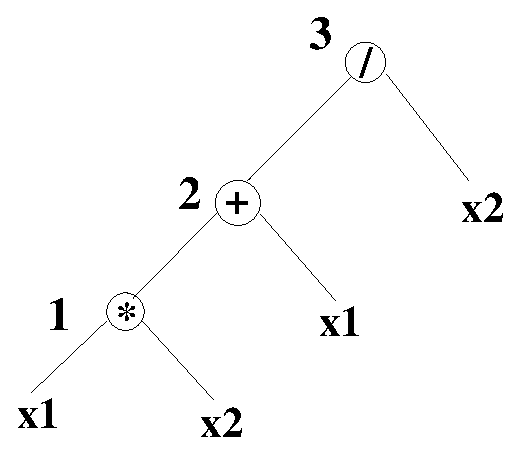
\includegraphics[scale=0.45]{Figs/fig2}
\caption[]{The parsing tree for $f(x_1,x_2)={x_1\times x_2+x_1 \over {x_2}}$}
\label{EX2}
\end{center}
\end{figure}
%\newpage
\begin{enumerate}
\item Stage {\bf 1}:
  
  The IDs of {\tt x$_1$} and {\tt x$_2$} are set to $0$ and $1$
  respectively and they are pushed on the \VMS.  {\tt x$_1$.rms()}
  and {\tt x$_2$.rms()} are copied in {\tt ME[0]} and {\tt ME[1]}
  respectively, while a value of $1$ is pushed on {\tt DS[0]} and {\tt
  DS[1]}.
  

  Operator {\tt '*'} pops two values (say {\tt L} and {\tt R}) from
  the \VMS.  A value {\tt L*R} with an ID equal to {\tt
  L.ID}$~\cup~${\tt R.ID} is pushed on the \VMS\ and a list of common
  IDs is made as {\tt IDList = L.IDList}$~\cap~${\tt R.IDList} (here,
  an empty list).  Next, for all IDs in {\tt L}, a value is poped from
  {\tt DS[L.ID]} (say, {\tt dx}), and {\tt dx*R} is pushed back on
  {\tt DS[L.ID]}.  Similar operation is done for all IDs in {\tt R}.
  
  Top of {\tt DS[0]} and {\tt DS[1]} now has {\tt x$_2$} and {\tt
  x$_1$} respectively, while the top of the \VMS\ has the value
  {\tt x$_1 \times $x$_2$} with an {\tt IDList=\{1,0\}}.

\item Stage {\bf 2}:
  
  {\tt x$_1$} is pushed on the \VMS, its ID is set to zero, {\tt
  x$_1$.rms()} is copied to {\tt ME[0]} (a redundant operation) and a
  value of $1$ is pushed on {\tt DS[0]}.
  
  Operator '{\texttt{+}}' pops two values ({\tt L} and {\tt R}) from the
  \VMS\ (these have values {\tt x$_1\times$x$_2$} and {\tt x$_1$}).
  {\tt L+R} with an {\tt IDList= L.ID}$~\cup~${\tt R.ID} is pushed
  back on the \VMS.  This {\tt IDList} will be {\tt \{0,1\}}.  For IDs
  common between {\tt L} and {\tt R} (here $\{0\}$), two values are
  poped from the \DS, and their addition pushed back on the \DS.  The
  common ID is then removed from the ID list of both operands.  For
  the remaining IDs in {\tt L} ({\tt R} has no IDs left), values are
  poped from the corresponding {\tt DS}, added together and pushed
  back on the appropriate {\tt DS}.
  
  Hence, at the end of the operator {\tt '+'}, {\tt DS[0]} will have
  {\tt x$_2$+1} and {\tt DS[1]} will have {\tt x$_1$}.  Top of the
  \VMS\ has the value {\tt x$_1 \times$x$_2$+x$_1$}.

\item Stage {\bf 3}:
  
  {\tt x$_2$} is pushed on the \VMS, {\tt x$_2$.rms()} is copied
  in {\tt ME[1]} (another redundant operation) and a value of $1$ is
  pushed on {\tt DS[1]}.
  
  Operator {\tt '/'} pops two values ({\tt L} and {\tt R}) from the
  \VMS.  A value of {\tt L/R} with an {\tt IDList=L.ID}$~\cup~${\tt
  R.ID} ($\{0,1\}\cup\{0\}$) is pushed on the \VMS.  A list of common
  IDs between {\tt L} and {\tt R} is made using {\tt IDList =
  L.IDList}$~\cap~${\tt R.IDList}.  For all IDs in {\tt IDList}, two
  values are poped from the corresponding {\tt DS} (say, {\tt dxR}
  ({\tt =x$_1$}) and {\tt dxL} (=1)) and {\tt (R*dxL -
  L*dxR)/(R*R)} pushed back on the same {\tt DS}.  The corresponding
  IDs are then removed from {\tt L} and {\tt R}.
  
  Next, for all the remaining IDs in {\tt L}, a value is poped (say
  {\tt dx}) from {\tt DS[L.ID]} and {\tt dx/R} is pushed back on the
  same {\tt DS}.  Similarly, for all IDs in {\tt R}, a value from {\tt
  DS[R.ID]} is poped into {\tt dx} and {\tt -L*dx/(R*R)} is pushed
  back on the same {\tt DS}.
  
  At the end of this stage, {\tt DS[0]} has the value {\tt 1+1/x$_2$}
  and {\tt DS[1]} has the value {\tt -x$_1$/x$_2^2$}.  \VMS\ now has
  ${{\tt x}_1 \times {\tt x}_2 + {\tt x}_1 \over {\tt x}_2}$.
       
\end{enumerate}

Finally, the values from the top of {\it all} {\tt DS}s are multiplied
with corresponding values in {\tt ME} table, squared, added and the
square root of the final result is taken.  That value will be
$\sqrt{\left[\left(1+{1\over {\tt x}_2}\right) \times \delta {\tt
x}_1\right]^2+\left[-{{\tt x}_1 \over {\tt x}_2^2} \times \delta {\tt
x}_2\right]^2}$.  This is the final error propagated through the
expression.

\section{Syntax}
\label{APPEN:SYNTAX}

This appendix describes the \Fussy\ syntax.  Statements are
interactively executed as soon as they are completed.  The virtual
code for the sub-programs (function or procedure) is held in the
memory and executed when the sub-programs are called.

\subsection{Numbers}
\label{NUMBERS}
Numbers in \Fussy\ are represented as floating point numbers and can
be specified with or without the decimal point, or in the exponent
format.  Optionally, an error can also be associated with the numbers
via the {\tt pm} directive.  E.g., $75.3\pm 10.1$ can be expressed as
{\tt 75.3pm10.1}.  Numbers can also be tagged with units (see
Section~\ref{UNITS}) or a {\tt C}-styled printing format (see
Section~\ref{FORMATTING}).

\subsubsection{Units}
\label{UNITS}
   
Numerical values can be specified along with their units.  As of now,
the only units supported are degree, arcmin, arcsec, hours, minute,
and seconds.  These can be specified by appending {\tt 'd', ''', '"',
'h', 'm', 's'} respectively to the numeric values.  Internally, all
numeric values are always stored in the MKS system of units.  The
default units for a variable used to specify angles or time is
radians.  If the values are specified along with any of the above
mentioned units, the values are still stored internally as radians.
However while printing (see Section~\ref{PRINT}), the values are
formatted automatically and printed with the appropriate units.

\subsection{Operators and built-in functions}

The normal binary operators of type {\tt expr <op> expr}, where {\tt
expr} is any expression/variable/constant and {\tt <op>} is one of
{\tt '+', '-', '/', '*'}, '{\texttt{\^}}' and {\tt '**'} binary
operators perform the usual mathematical operations in addition to
error propagation.  The comparison operators '{\texttt{<}}',
'{\texttt{>}}', '{\texttt{=}}', '{\texttt{!}}{\texttt{=}}',
'{\texttt{<}}{\texttt{=}}', '{\texttt{>}}{\texttt{=}}' and the logical
operators '{\texttt{|}}{\texttt{|}}' and '{\texttt{\&}}{\texttt{\&}}'
have the usual meaning.  Apart from the usual operation, the {\tt
var=expr} assignment operator also does the error propagation in the
expression on the RHS and assigns it as the error for the variable on
the LHS.  In addition to this, the assignment operator for partial
variables ({\tt pvar:=expr}) is also defined.  This does not propagate
the errors on the RHS but instead transfers all the required
information for error propagation to the variable on the LHS (see
Section~\ref{APPEN:SUBEXPRESSIONS}).  The result of these assignment
statements is the value of the variable on the LHS.  Hence expressions
like {\tt sin(x=0.1pm0.02)} are equivalent to {\tt
'x=0.1pm0.02;sin(x);'}.  The prefix and postfix operators {\tt
<op>var} and {\tt var<op>} where {\tt <op>} is either {\tt '++'} or
{\tt '--'} and {\tt var} is any user defined variable are also
defined.  These increment or decrement the value of the variables by
one.  The prefix and postfix operators operate on the variables before
and after the variable is further used respectively.

In addition, two operators of type {\tt expr.<op>} where {\tt <op>} is
either {\tt val} or {\tt rms} are also defined.  These operators
extract the value and the associated (propagated) error in {\tt expr}
which can be any mathematical expression or a variable.

%The following built-in functions are available: {\tt sin}, {\tt cos},
%{\tt tan}, {\tt asin}, {\tt acos}, {\tt atan}, {\tt atan2}, {\tt
%sinh}, {\tt cosh}, {\tt tanh}, {\tt asinh}, {\tt acosh}, {\tt atanh},
%{\tt exp}, {\tt ln}, {\tt log}, {\tt fabs}, {\tt fmod}, {\tt sqrt}
%{\tt int}.  The following functions, useful for astronomical
%computations are defined.  The latitude and longitude used for these
%computations are set in the global system variables {\tt LONGITUDE}
%and {\tt LATITUDE}.
%\begin{itemize}
%\item {\tt time()}:  returns the current time in the {\tt hms} format.
%\item {\tt lst()}:   returns the Local Sideral time in the {\tt hms} format.
%\item {\tt day()}:   returns the current day.
%\item {\tt month()}: returns the current month.
%\item {\tt year()}:  returns the current year.
%\item {\tt mjd(),fmjd()}: returns the current MJD and fractional MJD.
%\item {\tt setlong(MyLongitude)}: Sets the global variables {\tt LONGITUDE}
%to the given value.
%\item {\tt setlat(MyLatitude)}: Sets the global variables {\tt LATITUDE}
%to the given value.
%\end{itemize}

\subsection{Expressions/Statements}
\label{APPEN:SYNTAX_EXPR}

Numbers and variables can be combined with the mathematical operators
and logical operators to form an expression.  Expressions can be used
as arguments to built-in or user defined functions (see
Section~\ref{APPEN:SYNTAX_FUNC}).  An expression followed by a NEWLINE
prints its result on the output stream (see Section~\ref{PRINT}) in
the default format (see Section~\ref{FORMATTING}).

For the purpose of error propagation, the print statement and the
assignment operator (the ``{\tt =}'' operator but not the ``{\tt :=}''
operator; see Section~\ref{APPEN:SUBEXPRESSIONS}) are treated as the
terminal nodes of the parsing tree which invokes the final error
propagation.

Assigning a value to a variable also creates the variable.  The type
of the value assigned to the variable determines its type (and overrides
the value or the type of a previously declared variable).  E.g.
\begin{verbatim}
   >H_0=75pm10
   >H_0
             75.00000 +/-   10.00000
   >H_0="The Hubble constant\n"
   >H_0
    The Hubble constant
\end{verbatim}
A semi-colon ({\tt ';'}) is a delimiter to separate multiple
expressions in a single line.  Statements on separate lines need not
be delimited by semi-colons (though it is not an error to do so).
Compound statements are a group of simple statements, grouped using the
curly-brace pair ({\tt '\{'} and {\tt '\}'}) (e.g. {\tt \{a=1.5;
b=2;\}}). As may be obvious, compound statements can also be nested.
The {\tt '/\/*'} and {\tt '*/'} pair can be used as comment
delimiters.  Comment delimiters however cannot be nested. 
%E.g.

\subsection{Sub-expressions}
\label{APPEN:SUBEXPRESSIONS}

A special assignment operator '{\tt :=}' is used to assign
sub-expressions to user defined variables.  Sub-expression variables
are different from normal variables in that their propagated error is
computed on-the-fly when required, i.e.  when they are printed or are
assigned to a normal variable using the '{\tt =}' operator or at an
operator node of a parsing tree when used in another expression.  E.g.
\begin{verbatim}
   >x=1pm0.1
   >s:=sin(x);c:=cos(x);
   >sin(x)/cos(x) /* Compute tan(x) as sin(x)/cos(x) */
       1.55741 +/-    0.34255
   >s/c           /* Compute tan(x) using two PARTIAL_VAR */
       1.55741 +/-    0.34255
   >tan(x)        /* Direct computation of tan(x) */
       1.55741 +/-    0.34255
   >s2=s;
   >s2/c          /* Compute tan(x) with a normal variable
                     and one PARTIAL_VAR.  Error propagates 
                     differently */
       1.55741 +/-    0.26236
\end{verbatim}
\subsection{Variables and function/procedure names}

Variable/function/procedure names can be of any length and must match
the regular expression {\tt [a-zA-Z\_]+[a-zA-Z0-9\_]*}.  That is, the
names must start with an alphabet or {\tt '\_'} and can be followed by
one or more alpha-numeric characters or {\tt '\_'}.

\subsection{Function/procedure}
\label{APPEN:SYNTAX_FUNC}

Sub-programs can be written as functions or procedures.  The only
difference between functions and procedures is that functions {\it
must} return a value while procedures must {\it not} return a value.
The type of a sub-program which returns a value using the {\tt
return}~{\tt <expression>} statement becomes {\tt func}.  If {\tt
return} is not used, or is used without an {\tt expression}, the type
becomes {\tt proc}.  The type of the sub-program therefore need not be
declared.  It is an error to use a procedure in an expression or pass
a procedure as an argument to another sub-program where a function
should have been passed.

A function or procedure declaration begins with a variable name
followed by an argument list.  The argument list is enclosed by a
round bracket pair ({\tt '('} and {\tt ')'}).  A {\tt '()'} specifies
an empty argument list.  The function body is in enclosed between the
{\tt '\{'} and {\tt '\}'} brackets.  E.g.
\begin{verbatim}
   >/* An example of a funtion declaration */
   >f() { return sin(PI/2); }
   >/* An example of a procedure declaration */ 
   >p() {print "Value of f() = ",f(),"\n";}
   >f()
              1.00000
   >p() 
   Value of f() =    1.00000
\end{verbatim}
A sub-program can be passed as an argument to another sub-program.  An
argument corresponding to a sub-program can be specified using the
{\tt func} (for a function) or {\tt proc} (for a procedure) directive.
E.g.
\begin{verbatim}
   >f(x) { return sin(x); }
   >p(func fa,x) {print "The value of f(",x%5.2f,") =",fa(x),"\n";}
   >p(f,10)
   The value of f(10.00) =  -0.54402
\end{verbatim}
All symbols (variables, functions, procedures) used in the sub-program
code must be either global variables declared {\it before} the
sub-program declaration or must be one of the argument list.
Temporary variables, the scope of which is within the sub-program
only, can be declared using the {\tt auto} directive.  E.g.
\begin{verbatim}
   >f(x) { return sin(x); }
   >p(func fa,x)
     {
       auto t;
       t=fa(x);
       print "The value of f(",x%5.2f,") =",t,"\n";
     }
   >p(f,10)
   The value of f(10.00) =  -0.54402
\end{verbatim}


\subsection{Control statements}

The {\tt if-else}, {\tt while-} and {\tt for-}loops constitute the
program control statements.  These loops can be broken at any stage
with the use of the {\tt break} statement.  As of now, the conditions
which control the logic is evaluated ignoring the error with the
control variables.  Ultimately the goal is to provide a language
feature to specify a significance level and the conditional statements
return true if the error on the evaluated value is within the
significance level, else return false.

\subsubsection{{\tt if-else}}

The syntax for the {\tt if-else} statement is:
\begin{verbatim}
    if (condition)
       if-body-statment;

         or

    if (condition)
       if-body-statment else
       else-body-statment;
\end{verbatim}
The {\tt if-body-statement} and the {\tt else-body-statement} can be
any valid compound or simple statement.  In case of a simple
statement, the terminating semi-colon is necessary.

\subsubsection{{\tt while-loop}}

The syntax for the {\tt while-loop} is:
\begin{verbatim}
    while (condition)
       body-statment
\end{verbatim}
The {\tt body-statement} can be either a simple or a compound
statement and in case it is a simple statement, the terminating
semi-colon defines the end of the loop.

\subsubsection{{\tt for-loop}}

The syntax for the {\tt for-loop} is:
\begin{verbatim}
    for (init;condition;incr)
      body-statment
\end{verbatim}
where {\tt init} is a comma ({\tt ','}) separate list of simple
statements for initializing the loop variables.  E.g. {\tt init} can
be {\tt i=0,j=0,k=0}. {\tt condition} is a simple, single statement
while {\tt incr} is a list of comma separated statement(s). The {\tt
body-statement} can be any valid simple or compound statement.  {\tt
init} statements are executed first followed by the {\tt condition}
statement.  If the result of the {\tt condition} statement is non-zero
(logical true), the {\tt body-statements}, the {\tt incr} statement(s)
and the {\tt condition} statements are executed in a sequence till the
result of the {\tt condition} statement is zero (logical false).
E.g. following is a valid {\tt for-loop} with 3 loop-variables, only
one of which is checked in the condition:
\begin{verbatim}
    for (i=0,j=0,k=0;i<10;i=i+1,j=j+1;k=k+1) 
       print "i= ",i," j= ",j," k= ",k,"\n";
\end{verbatim}

\subsection{Print statement}
\label{PRINT}

The {\tt print} statement takes a comma separated list of objects to
be printed.  These objects can be quoted-strings, variables,
constants, condition statements or user defined function names.  The
list can consist of any number of objects and is terminated by a
semi-colon.  The format in which the numeric values are printed is
defined by the format modifier associated with the values (see
Section~\ref{FORMATTING}).  All escaped-characters used in C-styled
printing have the same effect as in the output of the C-styled {\tt
printf} statement.

\subsection{Formatting}
\label{FORMATTING}

Values can be formatted for printing in a variety of ways.  The format
in which a variable is printed is associated with the variable and
consists of a {\tt printf} styled formatting string (with extensions
for specifying the units of the numerical values as well).  E.g., if
{\tt x=75pm10}, by default {\tt x} will be printed using the {\tt
'\%10.5f'} format.  The default print format can be modified using the
{\tt '.'} operator on a variable.  E.g., one can fix the default print
format of {\tt x} to {\tt '\%5.2f'} by {\tt x.=\%5.2f}.

The print format of a value can also be temporarily modified by
specifying the format along with the variable/value.  E.g. the value
of {\tt x} can be printed in the exponent format as {\tt print x\%E}
or in the in hexadecimal format as {\tt print x\%x}.

An extra formatting, not available in {\tt printf} formatting, is that
of printing the individual bit values using the {\tt \%b} format.
With this, the value is printed in binary (1 or 0) format.  {\tt
\%B} does the same thing except that it prints a space after every 8 bits.
The value is casted into a {\tt unsigned long} integer before
printing.
\begin{verbatim}
   >x=10;x%B
        00000000 00000000 00000000 00001010
\end{verbatim}
If the units of a value are specified, the print format is also
appropriately modified.  If a variable has units of time or angle, its
print format is automatically set to {\tt \%hms} or {\tt \%dms}
and are printed in the {\tt XXhXXmXX.XXs} and {\tt
XXdXX{\texttt{'}}XX.XX{\texttt{"}}} styles respectively.


%\begin{acks}
\section*{ACKNOWLEDGEMENTS}
I thank D.~Oberoi and R.K.~Singh for many useful discussions.  This
work was started and largely done while I was working at the National
Center for Radio Astrophysics (NCRA), Pune of the Tata Institute of
Fundamental Research (TIFR), Mumbai, India and continued at my current
position at the National Radio Astronomy Observatory (NRAO), Socorro,
USA.  All of this work was done on computers running the GNU/Linux
operating system and I wish to thank the numerous contributors to this
software.
%\end{acks}

%\begin{thebibliography}{acmtrans}
%\bibliographystyle{acmtrans}
\bibliographystyle{aa}
\bibliography{fussy}
%\end{thebibliography}

%\begin{received}
%Received Nov. 2003; accepted Month Year
%\end{received}

%\endreceived

\end{document}
